\documentclass[conference,a4paper]{IEEEtran}

\usepackage{amsmath}
\newcommand{\beq}{\begin{equation}}
\newcommand{\eeq}{\end{equation}}
\newcommand{\sms}{\smallskip}
\newcommand{\ms}{\medskip}
\newcommand{\bs}{\bigskip}
\newcommand{\norm}[1]{\left\lVert#1\right\rVert}
\newtheorem{problem}{Problem}
\newtheorem{theorem}{Theorem}
\usepackage{graphicx}

% *** CITATION PACKAGES ***
%
%\usepackage{cite}
% cite.sty was written by Donald Arseneau
% V1.6 and later of IEEEtran pre-defines the format of the cite.sty package
% \cite{} output to follow that of the IEEE. Loading the cite package will
% result in citation numbers being automatically sorted and properly
% "compressed/ranged". e.g., [1], [9], [2], [7], [5], [6] without using
% cite.sty will become [1], [2], [5]--[7], [9] using cite.sty. cite.sty's
% \cite will automatically add leading space, if needed. Use cite.sty's
% noadjust option (cite.sty V3.8 and later) if you want to turn this off
% such as if a citation ever needs to be enclosed in parenthesis.
% cite.sty is already installed on most LaTeX systems. Be sure and use
% version 5.0 (2009-03-20) and later if using hyperref.sty.
% The latest version can be obtained at:
% http://www.ctan.org/pkg/cite
% The documentation is contained in the cite.sty file itself.






% *** GRAPHICS RELATED PACKAGES ***
%
\ifCLASSINFOpdf
  % \usepackage[pdftex]{graphicx}
  % declare the path(s) where your graphic files are
  % \graphicspath{{../pdf/}{../jpeg/}}
  % and their extensions so you won't have to specify these with
  % every instance of \includegraphics
  % \DeclareGraphicsExtensions{.pdf,.jpeg,.png}
\else
  % or other class option (dvipsone, dvipdf, if not using dvips). graphicx
  % will default to the driver specified in the system graphics.cfg if no
  % driver is specified.
  % \usepackage[dvips]{graphicx}
  % declare the path(s) where your graphic files are
  % \graphicspath{{../eps/}}
  % and their extensions so you won't have to specify these with
  % every instance of \includegraphics
  % \DeclareGraphicsExtensions{.eps}
\fi
% graphicx was written by David Carlisle and Sebastian Rahtz. It is
% required if you want graphics, photos, etc. graphicx.sty is already
% installed on most LaTeX systems. The latest version and documentation
% can be obtained at:
% http://www.ctan.org/pkg/graphicx
% Another good source of documentation is "Using Imported Graphics in
% LaTeX2e" by Keith Reckdahl which can be found at:
% http://www.ctan.org/pkg/epslatex
%






% *** MATH PACKAGES ***
%
%\usepackage{amsmath}
% A popular package from the American Mathematical Society that provides
% many useful and powerful commands for dealing with mathematics.
%
% Note that the amsmath package sets \interdisplaylinepenalty to 10000
% thus preventing page breaks from occurring within multiline equations. Use:
%\interdisplaylinepenalty=2500
% after loading amsmath to restore such page breaks as IEEEtran.cls normally
% does. amsmath.sty is already installed on most LaTeX systems. The latest
% version and documentation can be obtained at:
% http://www.ctan.org/pkg/amsmath





% *** SPECIALIZED LIST PACKAGES ***
%
%\usepackage{algorithmic}
% algorithmic.sty was written by Peter Williams and Rogerio Brito.
% This package provides an algorithmic environment fo describing algorithms.
% You can use the algorithmic environment in-text or within a figure
% environment to provide for a floating algorithm. Do NOT use the algorithm
% floating environment provided by algorithm.sty (by the same authors) or
% algorithm2e.sty (by Christophe Fiorio) as the IEEE does not use dedicated
% algorithm float types and packages that provide these will not provide
% correct IEEE style captions. The latest version and documentation of
% algorithmic.sty can be obtained at:
% http://www.ctan.org/pkg/algorithms
% Also of interest may be the (relatively newer and more customizable)
% algorithmicx.sty package by Szasz Janos:
% http://www.ctan.org/pkg/algorithmicx




% *** ALIGNMENT PACKAGES ***
%
%\usepackage{array}
% Frank Mittelbach's and David Carlisle's array.sty patches and improves
% the standard LaTeX2e array and tabular environments to provide better
% appearance and additional user controls. As the default LaTeX2e table
% generation code is lacking to the point of almost being broken with
% respect to the quality of the end results, all users are strongly
% advised to use an enhanced (at the very least that provided by array.sty)
% set of table tools. array.sty is already installed on most systems. The
% latest version and documentation can be obtained at:
% http://www.ctan.org/pkg/array


% IEEEtran contains the IEEEeqnarray family of commands that can be used to
% generate multiline equations as well as matrices, tables, etc., of high
% quality.




% *** SUBFIGURE PACKAGES ***
%\ifCLASSOPTIONcompsoc
%  \usepackage[caption=false,font=normalsize,labelfont=sf,textfont=sf]{subfig}
%\else
%  \usepackage[caption=false,font=footnotesize]{subfig}
%\fi
% subfig.sty, written by Steven Douglas Cochran, is the modern replacement
% for subfigure.sty, the latter of which is no longer maintained and is
% incompatible with some LaTeX packages including fixltx2e. However,
% subfig.sty requires and automatically loads Axel Sommerfeldt's caption.sty
% which will override IEEEtran.cls' handling of captions and this will result
% in non-IEEE style figure/table captions. To prevent this problem, be sure
% and invoke subfig.sty's "caption=false" package option (available since
% subfig.sty version 1.3, 2005/06/28) as this is will preserve IEEEtran.cls
% handling of captions.
% Note that the Computer Society format requires a larger sans serif font
% than the serif footnote size font used in traditional IEEE formatting
% and thus the need to invoke different subfig.sty package options depending
% on whether compsoc mode has been enabled.
%
% The latest version and documentation of subfig.sty can be obtained at:
% http://www.ctan.org/pkg/subfig




% *** FLOAT PACKAGES ***
%
%\usepackage{fixltx2e}
% fixltx2e, the successor to the earlier fix2col.sty, was written by
% Frank Mittelbach and David Carlisle. This package corrects a few problems
% in the LaTeX2e kernel, the most notable of which is that in current
% LaTeX2e releases, the ordering of single and double column floats is not
% guaranteed to be preserved. Thus, an unpatched LaTeX2e can allow a
% single column figure to be placed prior to an earlier double column
% figure.
% Be aware that LaTeX2e kernels dated 2015 and later have fixltx2e.sty's
% corrections already built into the system in which case a warning will
% be issued if an attempt is made to load fixltx2e.sty as it is no longer
% needed.
% The latest version and documentation can be found at:
% http://www.ctan.org/pkg/fixltx2e


%\usepackage{stfloats}
% stfloats.sty was written by Sigitas Tolusis. This package gives LaTeX2e
% the ability to do double column floats at the bottom of the page as well
% as the top. (e.g., "\begin{figure*}[!b]" is not normally possible in
% LaTeX2e). It also provides a command:
%\fnbelowfloat
% to enable the placement of footnotes below bottom floats (the standard
% LaTeX2e kernel puts them above bottom floats). This is an invasive package
% which rewrites many portions of the LaTeX2e float routines. It may not work
% with other packages that modify the LaTeX2e float routines. The latest
% version and documentation can be obtained at:
% http://www.ctan.org/pkg/stfloats
% Do not use the stfloats baselinefloat ability as the IEEE does not allow
% \baselineskip to stretch. Authors submitting work to the IEEE should note
% that the IEEE rarely uses double column equations and that authors should try
% to avoid such use. Do not be tempted to use the cuted.sty or midfloat.sty
% packages (also by Sigitas Tolusis) as the IEEE does not format its papers in
% such ways.
% Do not attempt to use stfloats with fixltx2e as they are incompatible.
% Instead, use Morten Hogholm'a dblfloatfix which combines the features
% of both fixltx2e and stfloats:
%
% \usepackage{dblfloatfix}
% The latest version can be found at:
% http://www.ctan.org/pkg/dblfloatfix




% *** PDF, URL AND HYPERLINK PACKAGES ***
%
%\usepackage{url}
% url.sty was written by Donald Arseneau. It provides better support for
% handling and breaking URLs. url.sty is already installed on most LaTeX
% systems. The latest version and documentation can be obtained at:
% http://www.ctan.org/pkg/url
% Basically, \url{my_url_here}.




% *** Do not adjust lengths that control margins, column widths, etc. ***
% *** Do not use packages that alter fonts (such as pslatex).         ***
% There should be no need to do such things with IEEEtran.cls V1.6 and later.
% (Unless specifically asked to do so by the journal or conference you plan
% to submit to, of course. )


% correct bad hyphenation here
\hyphenation{op-tical net-works semi-conduc-tor}


\begin{document}
   \IEEEoverridecommandlockouts
\IEEEpubid{\makebox[\columnwidth]{978-1-5090-0409-6/17/\$31.00~
\copyright2017 IEEE
 \hfill} \hspace{\columnsep}\makebox[\columnwidth]{ }}

%Also anywhere in the second column of your first page, please insert the
\IEEEpubidadjcol
%command to ensure that the bottom of the second column is correctly aligned.
%
% paper title
% Titles are generally capitalized except for words such as a, an, and, as,
% at, but, by, for, in, nor, of, on, or, the, to and up, which are usually
% not capitalized unless they are the first or last word of the title.
% Linebreaks \\ can be used within to get better formatting as desired.
% Do not put math or special symbols in the title.
\title{Novel method of informative frequency band selection for vibration signal using Nonnegative Matrix Factorization of Short-Time Fourier Transform}


% author names and affiliations
% use a multiple column layout for up to three different
% affiliations
\author{\IEEEauthorblockN{Jacek Wodecki, Piotr Kruczek\\and Agnieszka Wy{\l}oma{\'n}ska}
\IEEEauthorblockA{KGHM CUPRUM Ltd R$\&$D\\53-659 Wroc{\l}aw, Poland\\
Email: $\{$jwodecki,pkruczek,awylomanska$\}$\\@cuprum.wroc.pl}
\and
\IEEEauthorblockN{Anna Bartkowiak}
\IEEEauthorblockA{Institute of Computer Science\\Wroc{\l}aw University\\50-383 Wroc{\l}aw, Poland\\
Email: anna.bartkowiak@ii.uni.wroc.pl}
\and
\IEEEauthorblockN{Rados{\l}aw Zimroz}
\IEEEauthorblockA{Diagnostics and Vibro-Acoustics\\Science Laboratory,\\
Wroc{\l}aw University of Science\\and Technology, Wroc{\l}aw, Poland\\
Email: radoslaw.zimroz@pwr.edu.pl}}

% conference papers do not typically use \thanks and this command
% is locked out in conference mode. If really needed, such as for
% the acknowledgment of grants, issue a \IEEEoverridecommandlockouts
% after \documentclass

% for over three affiliations, or if they all won't fit within the width
% of the page, use this alternative format:
%
%\author{\IEEEauthorblockN{Michael Shell\IEEEauthorrefmark{1},
%Homer Simpson\IEEEauthorrefmark{2},
%James Kirk\IEEEauthorrefmark{3},
%Montgomery Scott\IEEEauthorrefmark{3} and
%Eldon Tyrell\IEEEauthorrefmark{4}}
%\IEEEauthorblockA{\IEEEauthorrefmark{1}School of Electrical and Computer Engineering\\
%Georgia Institute of Technology,
%Atlanta, Georgia 30332--0250\\ Email: see http://www.michaelshell.org/contact.html}
%\IEEEauthorblockA{\IEEEauthorrefmark{2}Twentieth Century Fox, Springfield, USA\\
%Email: homer@thesimpsons.com}
%\IEEEauthorblockA{\IEEEauthorrefmark{3}Starfleet Academy, San Francisco, California 96678-2391\\
%Telephone: (800) 555--1212, Fax: (888) 555--1212}
%\IEEEauthorblockA{\IEEEauthorrefmark{4}Tyrell Inc., 123 Replicant Street, Los Angeles, California 90210--4321}}




% use for special paper notices
%\IEEEspecialpapernotice{(Invited Paper)}




% make the title area
\maketitle

% As a general rule, do not put math, special symbols or citations
% in the abstract
\begin{abstract}
The problem of local damage detection in rotating machines is currently the highly important subject of interest. In the literature one can find many different strategies. One of the most common approaches is the vibration signal analysis aiming at informative frequency band selection. In case of simply structured signals classic methods (e.g. spectral kurtosis) are sufficient and return clear information about the damage. However, in real-world cases the signal is usually much more complicated. Indeed, such signals consist of many different components, for instance: damage-related cyclic impulses, high energy non-cyclic impulses not related to damage or heavy-tailed background noise etc. Hence, there is a growing need for robust damage detection methods. In this paper a novel method of informative frequency band selection is proposed. It utilizes the approach of Non-negative Matrix Factorization applied to time-frequency signal representation. The described algorithm is evaluated using simulated signal containing several different components, that resembles real-life vibration signal from copper ore crusher. Using the obtained structure of informative frequency band it is possible to filter particular components out of the original signal.
\end{abstract}

% no keywords




% For peer review papers, you can put extra information on the cover
% page as needed:
% \ifCLASSOPTIONpeerreview
% \begin{center} \bfseries EDICS Category: 3-BBND \end{center}
% \fi
%
% For peerreview papers, this IEEEtran command inserts a page break and
% creates the second title. It will be ignored for other modes.
\IEEEpeerreviewmaketitle



\section{Introduction}
Condition monitoring is highly important part of the maintenance of rotating machinery. One of the most common approaches is based on the analysis of the vibration signal. Recent methods for time-frequency analysis of rotating machinery is illustrated in \cite{feng2013recent,obuchowski2014recent}. Furthermore, the diagnostics of rolling elements bearing is described in details in \cite{randall2011rolling}. Interestingly, stochastic modelling methods are also powerful in case of condition monitoring. For instance, application of Schur filter \cite{Makowski2014130, lopatka2005effective} or autocorrelation and partial autocorrelation functions \cite{zak2014novel}.
The detection of damage can be also performed with selection of informative frequency band \cite{obuchowski2014selection}. The most classical approach is spectral kurtosis, which indicates the kurtosis for each frequency band in time-frequency representation of the signal \cite{antoni2006spectral, combet2009optimal}. In case of simple signal, which does not contain many different components spectral kurtosis is sufficient. On the other hand, in case of the machine working in harsh condition the condition monitoring is more complicated. Thus, the classical methods fail and the new approach should be proposed. One of the possible solution is an application of heavy tailed distribution, namely $\alpha$-stable distribution can be incorporated for informative band selection \cite{zak2016data}. Moreover, in case of the early stage of the damage another distribution can be applied. Indeed, the tempered stable distribution reveals an ability to detect smaller impulses \cite{wylomanska2016application}. In case of mining industry the working condition is harsh, there are many different sources of high energy noise. The contamination of vibration signal is high and cyclic impulses are hidden in the background noise. Therefore, the condition monitoring of the mining machinery is especially challenging \cite{bartelmus2014object}. The example of such machine is copper ore crusher. During the crushing process of big rocks high non-cyclic impulses are generated. The signal recorded on such machine was analysed in \cite{wylomanskaimpulsive}. The regime switching method for impulsive noise cancellation is used. As a result the signal component related to cyclic impulse is obtained. 

In this paper a different approach is proposed, that has been already studied in \cite{wodecki2017local}, namely the application of Non-negative Matrix Factorization (NMF) to the time-frequency representation of the signal. It has been shown that NMF is a powerful tool in data analysis and clustering \cite{cichocki2009nonnegative, zdunek2008data, wang2013nonnegative,lee1999learning, he2011symmetric}. In proposed algorithm, authors factorize the spectrogram matrix, which is squared absolute value of Short-Time Fourier Transform (STFT). Furthermore, as the result the filter characteristic is designed. In this article the method is tested for the signal, which contain cyclic and high energy non-cyclic impulses. It is expected that each of this signal components can be extracted from original waveform.

The rest of the paper is structured as follow. In Section \ref{sec:methodology} the methodology is introduced, the theory of NMF is recalled and the flowchart of the algorithm is presented. The application of the algorithm for simulated data is contained in Section \ref{sec:sim data}. Finally, the conclusion is presented in the last Section.

\section{Methodology}
\label{sec:methodology}
\subsection{Standard NMF with Euclidean objective}

Let $\bf{V}_{n\times m} $ denote an observed matrix {\bf  V} of
size $(n\times m)$ with non-negative elements. For such data matrix
${\bf V}$, Lee and Seung  proposed a factorization into two components \cite{lee2001algorithms}:
\beq\label{V1} {\bf V}_{n\times m}\simeq
      {\bf W}_{n\times r}*{\bf H}_{r\times m}. \eeq
      
     
All elements of the sought matrices ${\bf W}$ and ${\bf H}$ also have to be
non-negative, which is expressed by the constraints
\begin{align*}
    &v_{ij}\ge0,~~w_{ik}\ge 0,~~ h_{kj}\ge 0,\\
    &~~i=1, \dots, n; ~j=1,\dots, m;
                ~~k=1,\dots,r.
\end{align*}

The parameter $r$ is supposed to satisfy the in-equality: $r~<= min(n,m)$.
In the following, the parameter \emph{r} will represent the expected number of components in the signal.

The above formula says  that the original matrix \textbf{V} is
approximated by the product of two real-valued lower rank matrices: \emph{base matrix} ${\bf
W}_{n\times r}$ and \emph{encoding matrix} ${\bf H}_{r\times m}$  which have jointly less
elements than ${\bf V}$, i.e. the following inequality holds:
('$< <$' in (\ref{r1}) means: much smaller)

\begin{equation}\label{r1}
    (n+m)*r<\hspace{1pt}< n*m . 
\end{equation}

If truly formula (\ref{V1}) holds, which means, {\bf V} is well
approximated by the product {\bf W}*{\bf H}, then we may conclude that the
analyzed data matrix {\bf V} may be efficiently stored (and analyzed)
using only about (n+m)*r instead  of n*m data entries.

To approximately factorize $V\simeq{W*H}$, one should define cost function
that quantifies the approximation quality. It can be constructed
using distance measures between two matrices A and B. One of the most common and useful
measures is the square of the Euclidean distance:

\beq  
\norm{A-B}^2=\sum_{i,j}\left(A_{ij}-B_{ij} \right)
\eeq

Let us now consider an alternative formulation of such factorization as optimization problem: 
\newline
\begin{problem}
\label{prob:1}
Minimize $\norm{V-WH}^2$ with respect to $W$ and $H$, where $W,H \geq 0$
\end{problem}
~\\

The function $\norm{V-WH}^2$ is convex in terms of W or H exclusively, but not convex in both of them together. Hence, it is typically impossible to find global minima of the Problem 1. However, many optimization techniques can be applied to obtain them.
Perhaps the simplest one to implement is gradient descent, but its convergence is not very fast. Some other methods such as conjugate gradient converge quicker, at least in the neighbourhood of local minima, but are more complex to implement.

It has been determined by Lee and Seung that the following multiplicative update formulae are fast to compute and easy to implement for solving \ref{prob:1}:
\newline
\begin{theorem}
The Euclidean distance $\norm{V-WH}$ is non-increasing under the update rules 
\begin{equation}
    H_{\alpha\mu} \leftarrow H_{\alpha\mu}\frac{(W^TV)_{\alpha\mu}}{(W^TWH)_{\alpha\mu}} \quad
    W_{i\alpha} \leftarrow W_{i\alpha}\frac{(VH^T)_{i\alpha}}{(WHH^T)_{i\alpha}}
\end{equation}
\end{theorem}
~\\

In the practical implementation of the NMF algorithm matrix forms of presented equations have been used \cite{hoyer2004non}. Proof of convergence has been stated by Lee and Seung \cite{lee2001algorithms}. 

\subsection{Scope of the diagnostic algorithm}
\begin{figure}[!ht]
\centering
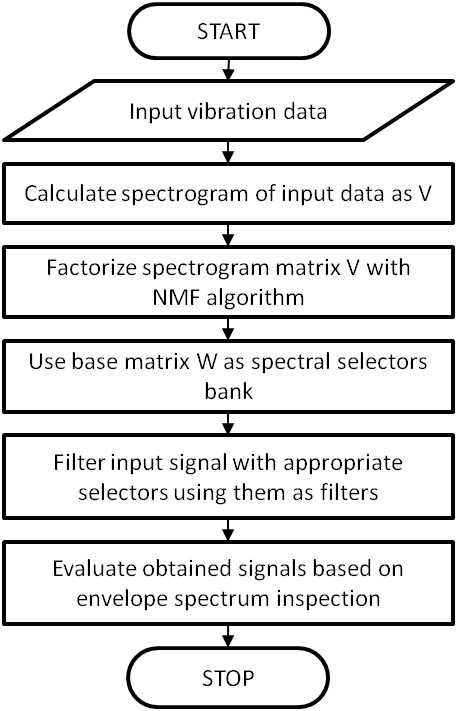
\includegraphics[width = 0.38\textwidth]{figs/block.png}
\caption{Flowchart of the diagnostic algorithm}
\label{fig: block}
\end{figure}

Functional flowchart of the proposed method is presented in Fig. \ref{fig: block}. Firstly, signal has to be transformed into a time-frequency domain. For such transformation spectrogram has been chosen, which is a square of absolute values of short-time Fourier transform (STFT), which for discrete data $x[0], x[1], ... , x[N-1]$ is defined as \cite{alan1989discrete}:

\begin{equation}
    \textrm{STFT}(n,k)=\sum_{m=0}^{L-1}x[n+m]w[m]e^{-j2\pi km/N},
\end{equation}
for $0\leq k \leq N-1$, and $w[.]$ is the window of length $L$. After that Nonnegative Matrix Factorization (NMF) algorithm is applied to extract spectral information about different types of processes occurring in the signal. As a result, $r$ selectors are obtained as column vectors of base matrix {\bf W}, where $r$ is the predefined expected number of processes. Finally, input signal is filtered with FFT-based FIR filter using overlap-add method, where given selector is used as filter transfer function \cite{alan1989discrete}. At the end, envelope spectra of obtained signals are calculated to inspect fundamental and harmonic frequencies of the components.

\section{Simulated data analysis}
\label{sec:sim data}
\subsection{Description of simulated data}

Simulated signal is a composite of cyclic impulses with a cyclic frequency of
40 Hz and carrier frequency band of $2500-3500$ Hz, noncyclic
impulses with a center frequency 5000 Hz and varying
bandwidths. The cyclic impulse is simulated using MATLAB
function \emph{gauspuls} with a center frequency $F_c = 3000$ Hz
and uniformly distributed bandwidth on
[0.2, 0.3] interval. As a next step, a single impulse is repeated to obtain cyclic signal. Non-cyclic impulse is also simulated using \emph{gauspuls} function
but with a centre frequency $F_c = 5000$ Hz and uniformly distributed bandwidth on [0, 1] interval. Positions of the non-cyclic impulses are uniformly distributed
on the time axis. The model of the simulated signal is presented in Fig. \ref{fig:schemat sygnal}.

\begin{figure}[ht!]
    \centering
    \includegraphics[width = 0.48\textwidth]{figs/schemat.png}
    \caption{The schematic model of the signal}
    \label{fig:schemat sygnal}
\end{figure}

\subsection{Results}

Time series of simulated vibration data is presented in Fig. \ref{fig: input}. This data has been already addressed in \cite{wylomanskaimpulsive}, where other methods of IFB estimation have been described. Spectrogram is obtained for Hamming 256-sample length window with 220 samples overlapping and 512 FFT points. One can observe several strong, non-cyclic excitations emerging from the noise, but no cyclic impulses are visible. Even on spectrogram they are not very obviously noticeable (see Fig. \ref{fig: spectrogram}).

\begin{figure}[!ht]
%\vspace{-10pt}
\centering
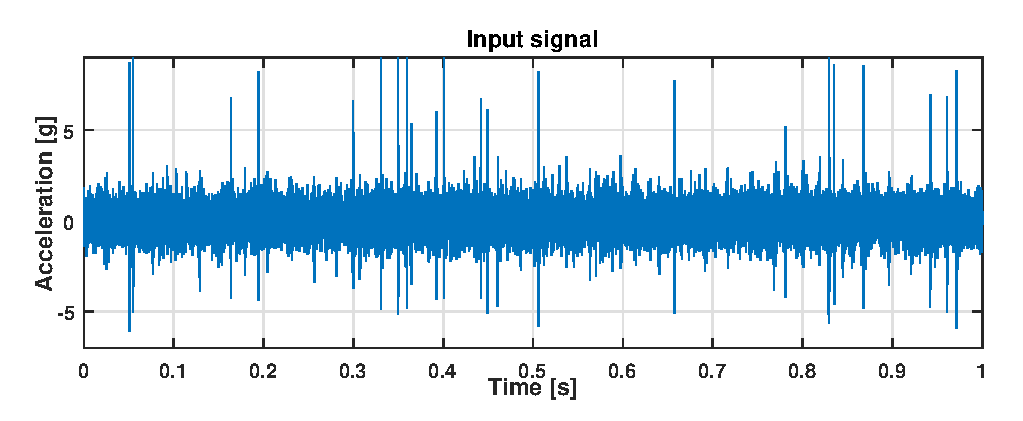
\includegraphics[width = 0.48\textwidth]{figs/input_sig.eps}
\caption{Simulated input signal}
\label{fig: input}
\end{figure}

\begin{figure}[!ht]
\centering
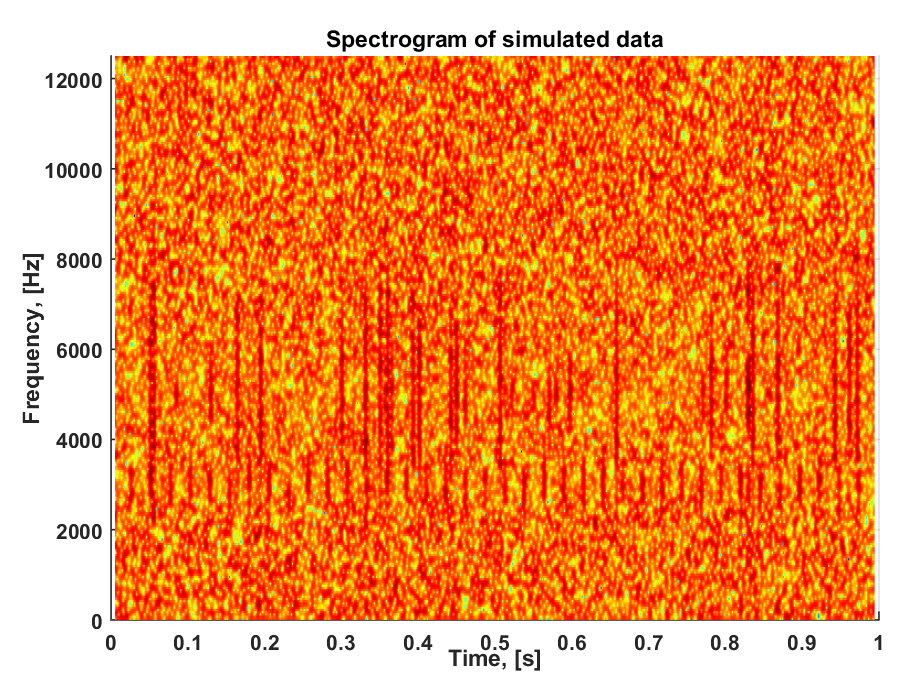
\includegraphics[width = 0.48\textwidth]{figs/input_spec.eps}
\caption{Time-frequency representation of the input signal}
\label{fig: spectrogram}
\end{figure}

As a next step, NMF algorithm differentiates spectral profiles of previously described processes (see Fig. \ref{fig: selmat}). Based on the visual inspection of the spectrogram matrix, one can recognise that second cluster describes spectrum of cyclic impulsive component, and third component is responsible for the non-cyclic process.

\begin{figure}[!ht]
\centering
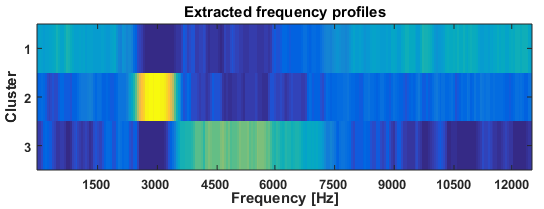
\includegraphics[width = 0.48\textwidth]{figs/selector_matrix.png}
\caption{Matrix of IFB selectors obtained by NMF}
\label{fig: selmat}
\end{figure}

Selectors used as transfer functions for the filtration step are presented in Fig. \ref{fig: selplots}. 

\begin{figure}[!ht]
\centering
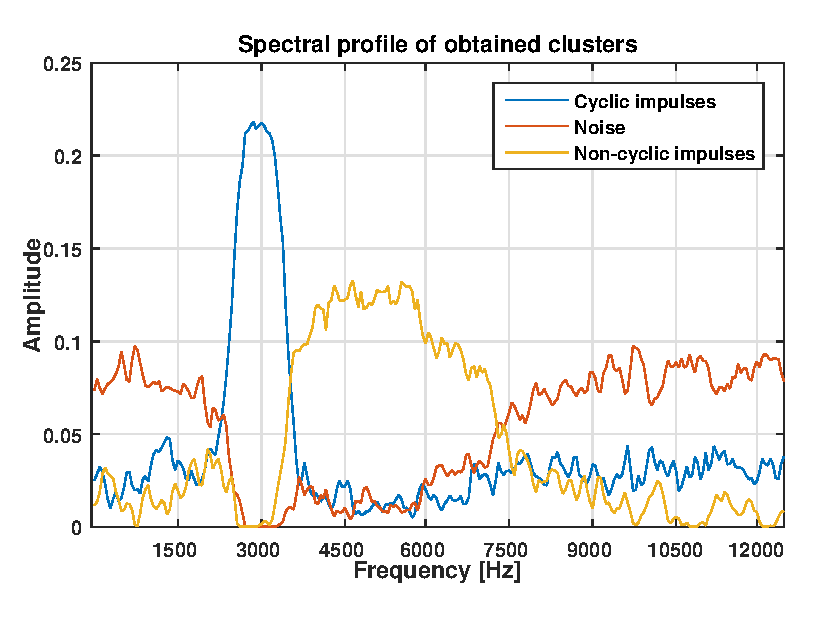
\includegraphics[width = 0.48\textwidth]{figs/selector_plot.eps}
\caption{Plot of IFB selectors for three components}
\label{fig: selplots}
\end{figure}

Input signal (Fig. \ref{fig: outplots} a) has been filtered with two selectors extracting non-cyclic and cyclic components (Fig. \ref{fig: outplots} b and c respectively). Obtained signals carry information about random impacts being natural behavior of this type of machines, and cyclic impulsive process that denotes detected local damage.

\begin{figure}[!ht]
\centering
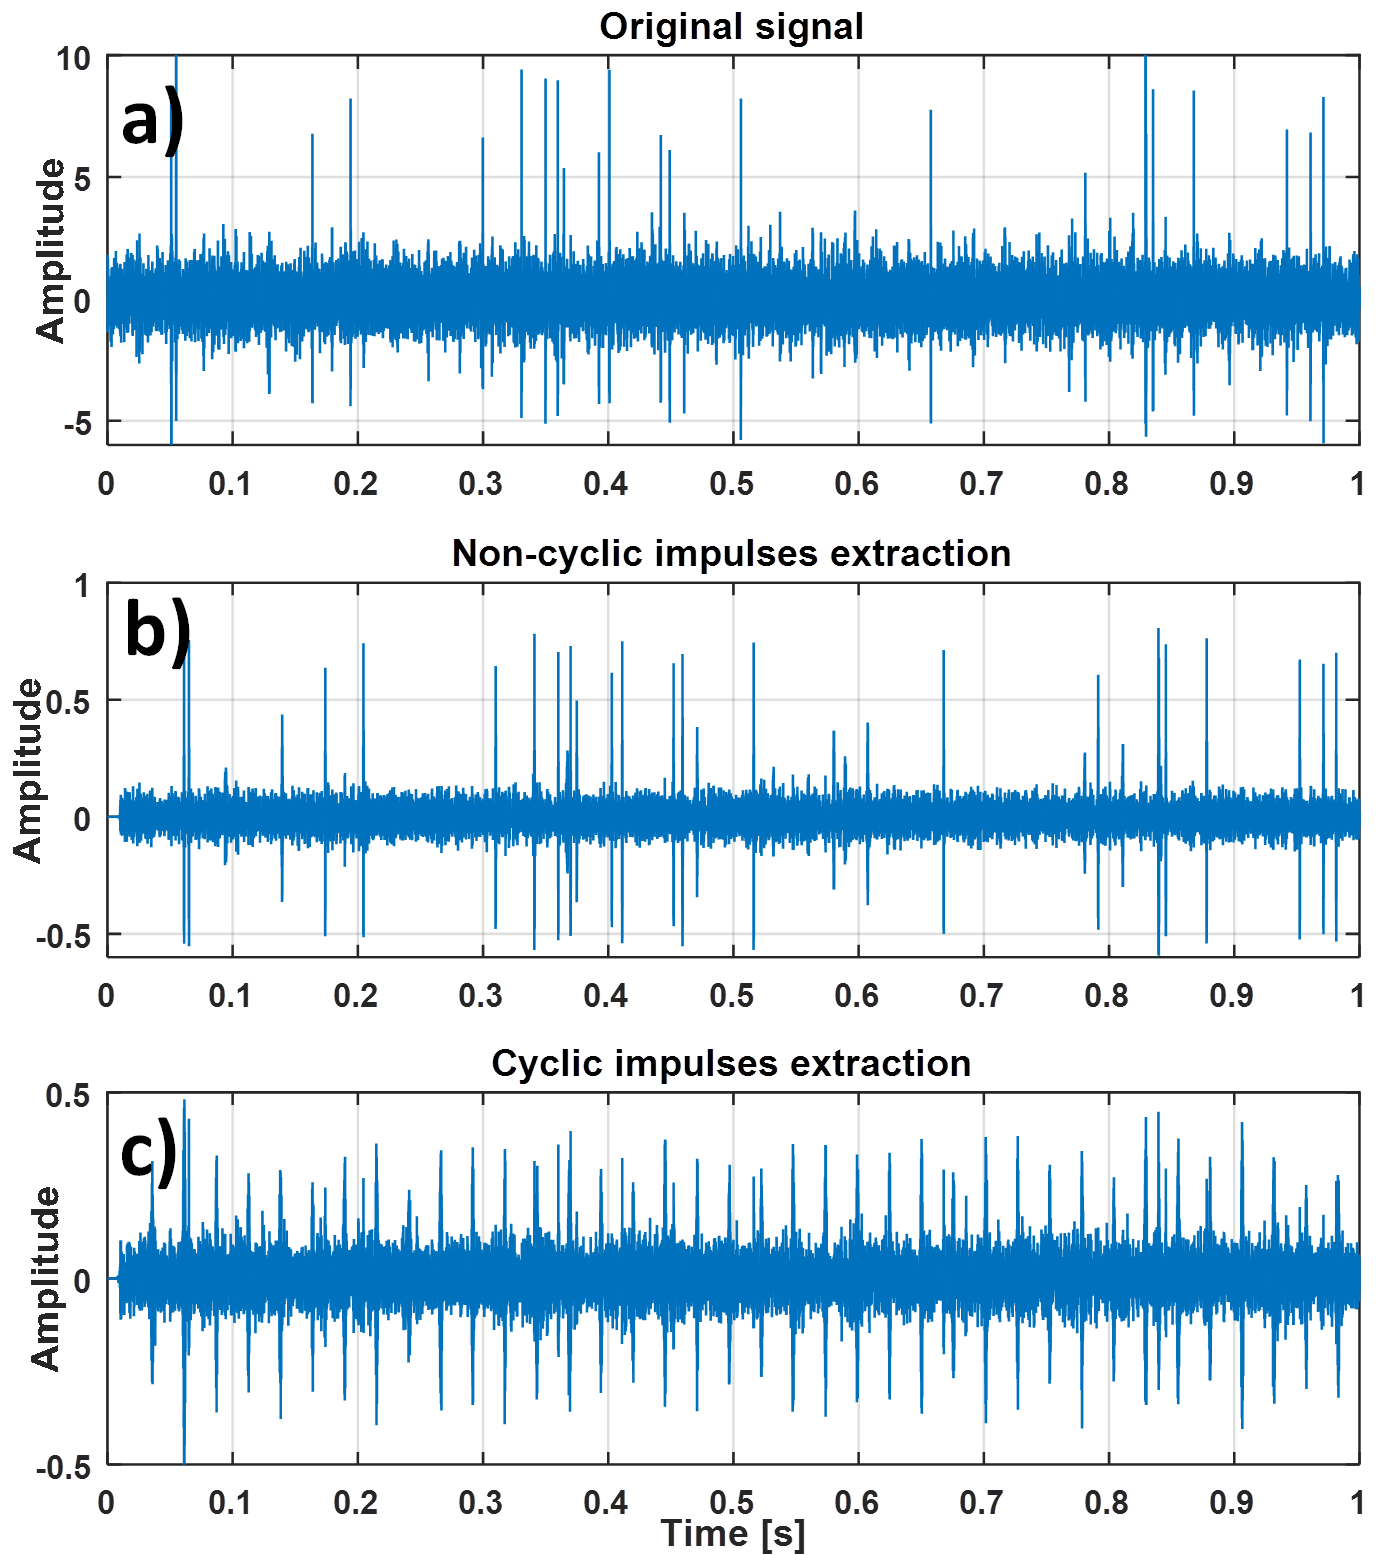
\includegraphics[width = 0.48\textwidth]{figs/output_plots.png}
\caption{Results of filtration: a) original signal, b) non-cyclic impulses, c) cyclic impulses}
\label{fig: outplots}
\end{figure}

\begin{figure}[!ht]
\centering
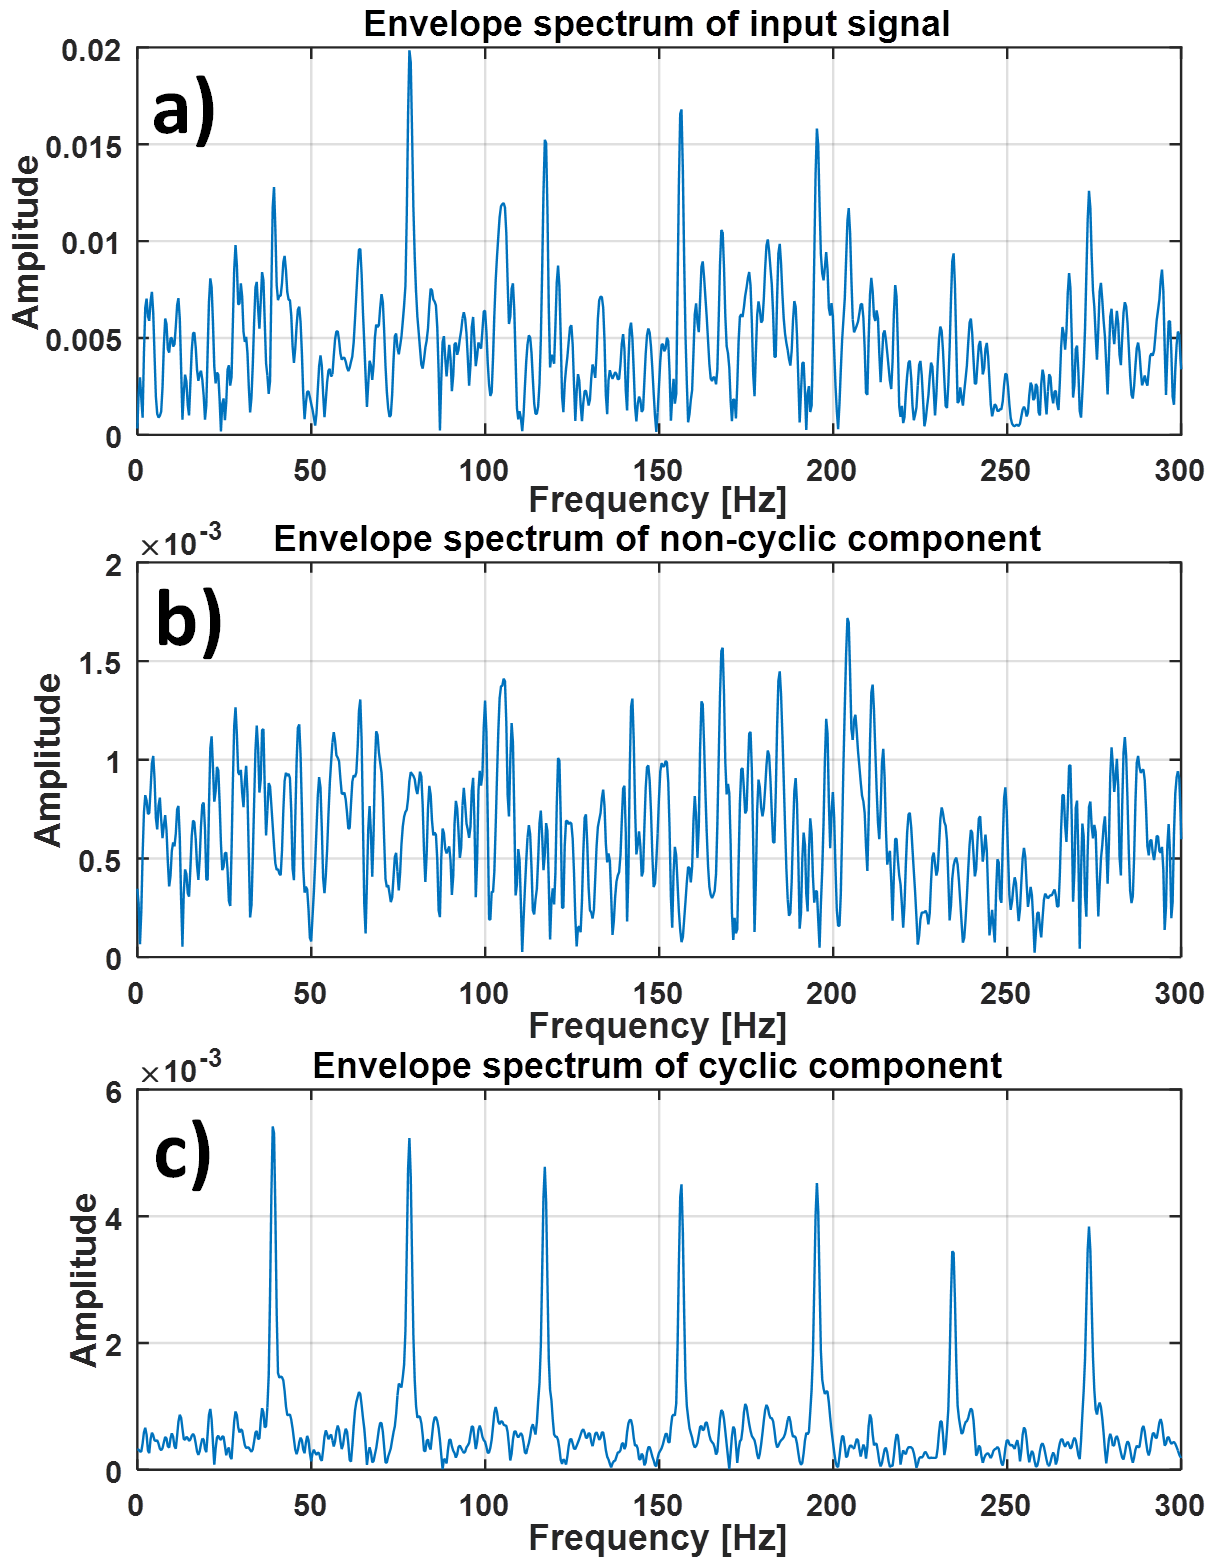
\includegraphics[width = 0.48\textwidth]{figs/output_specs2.png}
\caption{Envelope spectra of the results: a) original signal, b) non-cyclic impulses, c) cyclic impulses}
\label{fig: outspecs}
\end{figure}

In addition, quality and clarity of obtained components can be evaluated using envelope spectra (see Fig. \ref{fig: outspecs}). Spectrum of input signal (panel a) provides no conclusive information about the damage. Although there are several visible peaks in the spectrum, their presence and meaning is questionable. Envelope spectrum of non-cyclic component (panel b) looks random, which is expected effect because of randomness of impulses' bandwith and position in time domain. Finally, envelope spectrum of cyclic component (panel c) provides unquestionable series of peaks at fundamental and harmonic frequencies related to local damage (in this case 40 Hz and its multiples). 
% An example of a floating figure using the graphicx package.
% Note that \label must occur AFTER (or within) \caption.
% For figures, \caption should occur after the \includegraphics.
% Note that IEEEtran v1.7 and later has special internal code that
% is designed to preserve the operation of \label within \caption
% even when the captionsoff option is in effect. However, because
% of issues like this, it may be the safest practice to put all your
% \label just after \caption rather than within \caption{}.
%
% Reminder: the "draftcls" or "draftclsnofoot", not "draft", class
% option should be used if it is desired that the figures are to be
% displayed while in draft mode.
%
%\begin{figure}[!t]
%\centering
%\includegraphics[width=2.5in]{myfigure}
% where an .eps filename suffix will be assumed under latex,
% and a .pdf suffix will be assumed for pdflatex; or what has been declared
% via \DeclareGraphicsExtensions.
%\caption{Simulation results for the network.}
%\label{fig_sim}
%\end{figure}

% Note that the IEEE typically puts floats only at the top, even when this
% results in a large percentage of a column being occupied by floats.


% An example of a double column floating figure using two subfigures.
% (The subfig.sty package must be loaded for this to work.)
% The subfigure \label commands are set within each subfloat command,
% and the \label for the overall figure must come after \caption.
% \hfil is used as a separator to get equal spacing.
% Watch out that the combined width of all the subfigures on a
% line do not exceed the text width or a line break will occur.
%
%\begin{figure*}[!t]
%\centering
%\subfloat[Case I]{\includegraphics[width=2.5in]{box}%
%\label{fig_first_case}}
%\hfil
%\subfloat[Case II]{\includegraphics[width=2.5in]{box}%
%\label{fig_second_case}}
%\caption{Simulation results for the network.}
%\label{fig_sim}
%\end{figure*}
%
% Note that often IEEE papers with subfigures do not employ subfigure
% captions (using the optional argument to \subfloat[]), but instead will
% reference/describe all of them (a), (b), etc., within the main caption.
% Be aware that for subfig.sty to generate the (a), (b), etc., subfigure
% labels, the optional argument to \subfloat must be present. If a
% subcaption is not desired, just leave its contents blank,
% e.g., \subfloat[].


% An example of a floating table. Note that, for IEEE style tables, the
% \caption command should come BEFORE the table and, given that table
% captions serve much like titles, are usually capitalized except for words
% such as a, an, and, as, at, but, by, for, in, nor, of, on, or, the, to
% and up, which are usually not capitalized unless they are the first or
% last word of the caption. Table text will default to \footnotesize as
% the IEEE normally uses this smaller font for tables.
% The \label must come after \caption as always.
%
%\begin{table}[!t]
%% increase table row spacing, adjust to taste
%\renewcommand{\arraystretch}{1.3}
% if using array.sty, it might be a good idea to tweak the value of
% \extrarowheight as needed to properly center the text within the cells
%\caption{An Example of a Table}
%\label{table_example}
%\centering
%% Some packages, such as MDW tools, offer better commands for making tables
%% than the plain LaTeX2e tabular which is used here.
%\begin{tabular}{|c||c|}
%\hline
%One & Two\\
%\hline
%Three & Four\\
%\hline
%\end{tabular}
%\end{table}


% Note that the IEEE does not put floats in the very first column
% - or typically anywhere on the first page for that matter. Also,
% in-text middle ("here") positioning is typically not used, but it
% is allowed and encouraged for Computer Society conferences (but
% not Computer Society journals). Most IEEE journals/conferences use
% top floats exclusively.
% Note that, LaTeX2e, unlike IEEE journals/conferences, places
% footnotes above bottom floats. This can be corrected via the
% \fnbelowfloat command of the stfloats package.




\section{Conclusion}
In this paper authors introduce new method of local damage detection in rotating machinery. Although the idea of selectors is widely known, it is proposed to perform Nonnegative Matrix Factorization of the spectrogram matrix and use base matrix as a selector bank. Analyzed data filtered with obtained selectors reveal the underlying component processes occurring in the signal, most important being the cyclic impulsive component related to local damage. Differentiation of spectral structure allows to properly distinguish particular classes of existing processes.




% conference papers do not normally have an appendix


% use section* for acknowledgment
\section*{Acknowledgment}
This work is partially (J. Wodecki, P. Kruczek, A. Wy{\l}oma{\'n}ska) supported by the Framework Programme for Research and Innovation Horizon 2020 under grant agreement n. 636834 (DISIRE - Integrated Process Control based on Distributed In-Situ Sensors into Raw Material and Energy Feedstock) 

The work is supported by the Statutory Grant no.0401/0166/16 (Rados{\l}aw Zimroz)





% trigger a \newpage just before the given reference
% number - used to balance the columns on the last page
% adjust value as needed - may need to be readjusted if
% the document is modified later
%\IEEEtriggeratref{8}
% The "triggered" command can be changed if desired:
%\IEEEtriggercmd{\enlargethispage{-5in}}

% references section

% can use a bibliography generated by BibTeX as a .bbl file
% BibTeX documentation can be easily obtained at:
% http://mirror.ctan.org/biblio/bibtex/contrib/doc/
% The IEEEtran BibTeX style support page is at:
% http://www.michaelshell.org/tex/ieeetran/bibtex/
%\bibliographystyle{IEEEtran}
% argument is your BibTeX string definitions and bibliography database(s)
%\bibliography{IEEEabrv,../bib/paper}
%
% <OR> manually copy in the resultant .bbl file
% set second argument of \begin to the number of references
% (used to reserve space for the reference number labels box)

\bibliographystyle{IEEEtran}
\bibliography{mybib}

% \begin{thebibliography}{1}

% \bibitem{IEEEhowto:kopka}
% H.~Kopka and P.~W. Daly, \emph{A Guide to \LaTeX}, 3rd~ed.\hskip 1em plus
%   0.5em minus 0.4em\relax Harlow, England: Addison-Wesley, 1999.

% \end{thebibliography}

\textbf{Jacek Wodecki} received the M.Sc. degree in Electronics from the Faculty of Electronics on Wroclaw University of  Science and Technology, Wroclaw, Poland. PhD student in Diagnostics and Vibro-Acoustic Science Laboratory at Faculty of Geoengineering, Mining and Geology at Wroclaw University of Science and Technology. Works at KGHM CUPRUM R\&D Ltd. Areas of interest: multivariate data analysis, multidimensional signal processing and machine learning.

\textbf{Piotr Kruczek} received the M.Sc. degree in Mathematics for Industry and Commerce from Institute of Mathematics and Computer Science at the Wroclaw University of Science and Technology. Currently, PhD student in Faculty of Pure and Applied Mathematics at Wroclaw University of Science and Techonology. Works at KGHM CUPRUM R\&D Ltd. He is areas of interested are focused on condition monitoring, data analysis and time series analysis.

\textbf{Anna Bartkowiak} has received her MSc and PhD degrees in Applied Mathematics from the University of Wroclaw, Poland,  and her DSc degree (habilitation) from the Institute of Computer Science, Polish Academy of Sciences Warsaw, Poland. She is presently Professor Emeritus in the Institute of Computer Science, University of Wroclaw. She is a member of the International Biometrical Society (IBS),  a Fellow of the Royal Statistical Society (RSS), London;  a member of the American Statististical Society (ASA), also a member of the International Association for Statistical Computing (IASC ISI), and a member of the Polish	Information Processing Society (PTI). Her scientific interests are: algorithms of computational statistics and  multivariate analysis with graphical visualization of observational data. She has published -- in Polish -- several books on these topics. She has also published -- in English , in international journals and international conference proceedings -- more than 200 papers on the mentioned topics of her interests.

\textbf{Agnieszka Wylomanska} received the M.Sc. degree in Financial and Insurance Mathematics from Institute of Mathematics and Computer Science at the Wroclaw University of Science and Technology (WUST, Poland)  in 2002, the Ph.D. degree in Mathematics from WUST in 2006 and the D.Sc. degree in Mining and Engineering Geology from Faculty of Geoengineering, Mining and Geology (WUST, 2015). In the period 2007-2015 she was an Assistant Professor with the Faculty of Fundamental Problems of Technology, WUST. Currently she is Assistant Professor with the Faculty of Pure and Applied Mathematics and a member of the Hugo Steinhaus Center for stochastic processes. Her area of interest relates to time series analysis, stochastic modeling and statistical analysis of real data (especially technical data related to vibration signals and indoor air quality time series). She is an author of more than 90 research papers.

\textbf{Radoslaw Zimroz} received the M.Sc. degree in Acoustics from Institute of Telecommunication and Acoustics, Wroclaw University of Science and Technology, Poland (1998), the Ph.D. and the D.Sc. degrees in Mining and Geology from Faculty of Mining (WUST, 2002,2011, respectively). Since 2012 he serves as Professor and head of VibroAcoustic and Diagnostic Laboratory in this faculty. His area of interest relates to model based and industrial Condition Monitoring of mining machines including such topics as signal acquisition systems, signal processing, multidimensional data analysis, adaptive decision making, especially in the context of non-stationary operating conditions. He is author of more than 200 works with over 40 published in leading journals and indexed conference proceedings.


% that's all folks
\end{document}


